\input{permve-ntnu-latex-assignment.tex}

\usepackage{float}
\usepackage{tabularx}

\title{
\normalfont \normalsize
\textsc{Norwegian University of Science and Technology\\IT3105 -- Artificial Intelligence Programming}
\horrule{0.5pt} \\[0.4cm]
\huge Module 6:\\ Deep Learning for Game Playing\\
\horrule{2pt} \\[0.5cm]
}

\author{Per Magnus Veierland\\permve@stud.ntnu.no}

\date{\normalsize\today}

\newacro{ANN}{Artificial Neural Network}
\newacro{SGD}{Stochastic Gradient Descent}

\begin{document}

\fancyfoot[C]{}
\maketitle

\newpage
\fancyfoot[C]{\thepage~of~\pageref{LastPage}} % Page numbering for right footer
\setcounter{page}{1}

\section*{Knowledge Representation}

The goal of the module is to find a way to train an \ac{ANN} with supervised learning such that it can beat a random player at the game \textsc{2048}. The assignment states the difficulty of this task clearly, and heavily suggests preprocessing the board state to expose features in a form which is easier to learn by the network.

Based on this, two preprocessing schemes has been developed to transform a board state into features which are used as inputs to the \ac{ANN}. To construct the training data for the two schemes, an evaluation function is needed to decide which move to choose for each network input when generating training data.

During prototyping, a small reference algorithm was written in Python to find a set of working features upon which to base a heuristic for satisfactory play. An important factor when doing supervised learning is that the answer in training examples must correspond well to the inputs presented in the training example. It was found when building the reference implementation that greedily selecting the move which maximizes the number of open cells will result in a mean score of $\approx 230$, which significantly beats the mean random play score of $\approx 110$ (see Table~\ref{table:results}). This same heuristic is used to produce the correct move for both approaches.

The first knowledge engineering approach is the most basic of the two and involves feeding the number of possible merges for each row and each column in the current state as inputs to the network; resulting in 8 network inputs. Intuitively this should work well, as the information of how many merges are possible in each direction should be sufficient to correctly chose the optimal move according to the heuristic of maximizing the number of free cells.

The second knowledge engineering approach is more complex. An obvious solution would be to feed the board state directly into the network. However, this representation is complex and involves a range of different values for each cell. In an effort to simplify the board input, while allowing the network to learn when cells can be merged, a reduction is performed on the input values. For a given board state, the number of distinct non-zero values in the state is first counted. If a row in the board state has the values \texttt{[0 2 4 2]}, then the row has two distinct non-zero values. After counting the number of non-zero values, each non-zero value on the board is reassigned to be its equal to its index in the sorted list of unique non-zero values. This reduction is meant to make the network blind to the magnitude of values in a board state and only treat values according to mergeability. The number of network inputs for the second approach is 16, corresponding to the reduced board cell values.

An important detail when producing training examples was to leave out examples where the heuristic was not able to distinguish one move as better than any other move. Unless the heuristic clearly knows that one move is the right move for the given state, it is assumed to not be beneficial to insist that the training examples follows the same ``random'' move that the example generator ends up making.

\begin{table}
\centering
{\small
\begin{tabular}{ccccccc}
\toprule
Player    & Dimensions                          & Hidden $f$    & Output $f$       & $\varepsilon$ [\%] & Mean score & $\sigma~\text{score}$ \\
\midrule
Random    & N/A                                 & N/A           & N/A              & N/A                & 107.26     &  54.4479              \\
Reference & N/A                                 & N/A           & N/A              & N/A                & 231.87     & 125.5831              \\
Network A & $8 \times 4$                        & \textsc{ReLu} & \textsc{Softmax} & 0.0000             & 250.56     & 129.0481              \\
Network B & $16 \times 512 \times 512 \times 4$ & \textsc{ReLu} & \textsc{Softmax} & 0.2563             & 221.31     & 117.8580              \\
\bottomrule
\end{tabular}
}
\caption{Statistics comparing the two chosen networks and the reference implementation. All networks use cross-entropy cost functions and are trained with learning~rate~0.08. Network~A is trained with minibatch size 40 and network~B with minibatch size 50. All scores are based on highest tile present at end of game; averaged over 1000 games. $\varepsilon~=~\text{Training set error}$. $\sigma~=~\text{standard deviation}$.}
\label{table:results}
\end{table}

\section*{Network Design}

The network inputs chosen for both representations has the same range in each representation. By using the \textit{rectifier} activation function, scaling the inputs is not required as the activation function cannot be saturated, and because all values will be close to zero already. The \textit{softmax} function is used for the output nodes to rank the most probable move.

The first network using the basic knowledge representation scheme does not require any hidden layer. It is able to train to 0\% error within the first couple of epochs. It is however necessary to provide a large enough number of training examples. With training examples based on 100 games played a training error of 0\% was not achieved. However, increasing the number of training examples to 1000 games was sufficient to complete optimal training. It is clear that the first knowledge representation scheme requires little ``intelligence'' from the network. This is intuitive, as it should be straightforward to select an optimal move to maximize the number of free cells based on the number of possible merges for each row and column.

The second network requires a much larger topology. Achieving good training errors required large hidden layers, and the final network uses two hidden layers of 512 nodes each. It is possible to train a network to achieve a training error of 0 since the preprocessing used for the first network is a simple algorithm. However this will likely require more training data and possibly even larger topology.

Both networks use \textit{softmax} output nodes and the cross-entropy loss function as these yielded good results for the MNIST dataset in module~5.

Running each trained network for 1000 games and running a \textit{Welch}-test produces a $p$-value of 0.0. It is clear that network~A with the much simpler input and topology beats network~B with the more complex input and topology. It is also clear that the choices and reduction algorithm used to produce feature input to the more complex network produces good results which could be improved further with the same input.

\section*{Play Analysis}

Both network configurations and their associated preprocessing stages are able to approximate the heuristic function well by achieving a low training error. When the training error is 0, bad moves will either occur because the training set is not large enough for the \ac{ANN} to capture the information necessary to model the heuristic function -- or because the heuristic function simply made an evaluation with poor results.

During observed play bad moves were only seen which were caused by the simplistic heuristic function chosen.

\begin{figure}[!h]
\centering
\begin{tabularx}{\textwidth}{cXc}
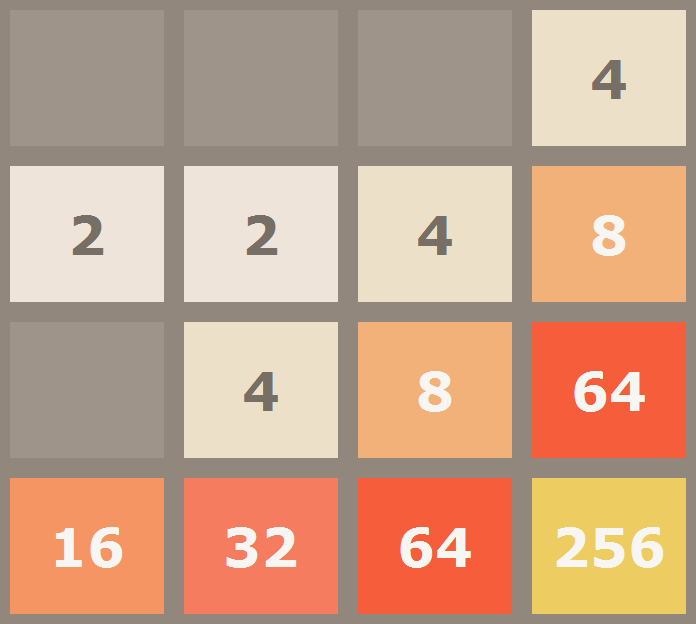
\includegraphics[scale=0.35]{bad_1} & ~ & 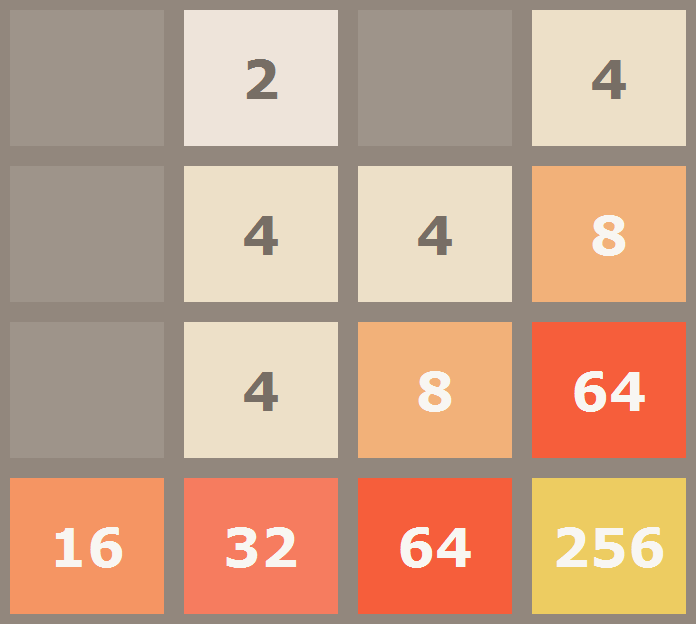
\includegraphics[scale=0.35]{bad_2} \\
\end{tabularx}
\caption{\textit{Example of poor gameplay:} Instead of moving up to gather the 4-tile, the 8-tile and the 16-tile to the right -- while keeping the 2-tiles to the upper left gathered -- the \ac{ANN} instead choses to greedily merge two 2-tiles while risking worsening the board state by permitting tiles to spawn at the top of the board.}
\label{fig:N1}
\end{figure}
\begin{figure}[!h]
\centering
\begin{tabularx}{\textwidth}{cXc}
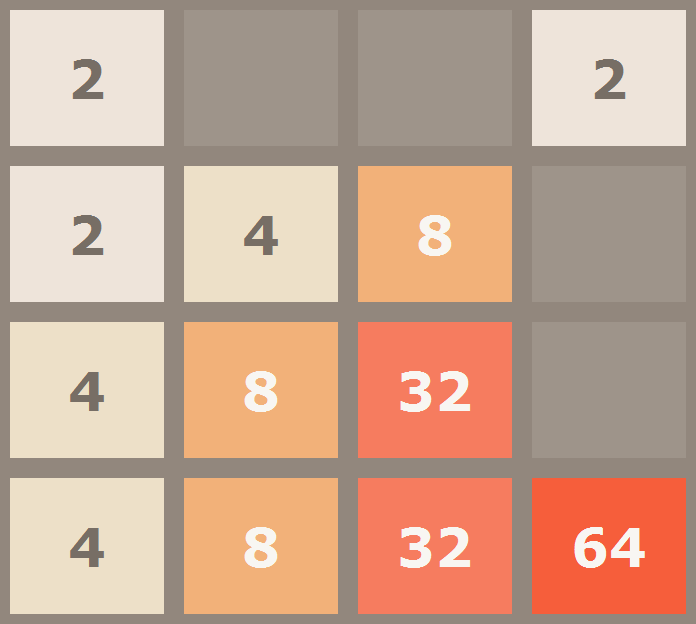
\includegraphics[scale=0.35]{good_1} & ~ & 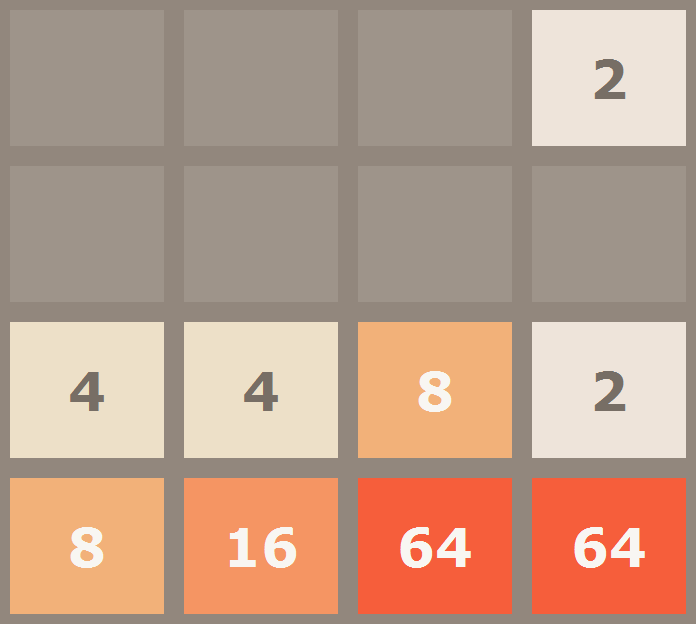
\includegraphics[scale=0.35]{good_2} \\
\end{tabularx}
\caption{\textit{Example of good gameplay:} In this scenario the board state offers the possibility to merge four tile pairs. The greedy heuristic which the \ac{ANN} models recognizes this possibility and performs four simultaneous merge while at the same time lining up two new merges.}
\label{fig:N1}
\end{figure}

\end{document}

